\begin{figure*}[t!]
    \centering
        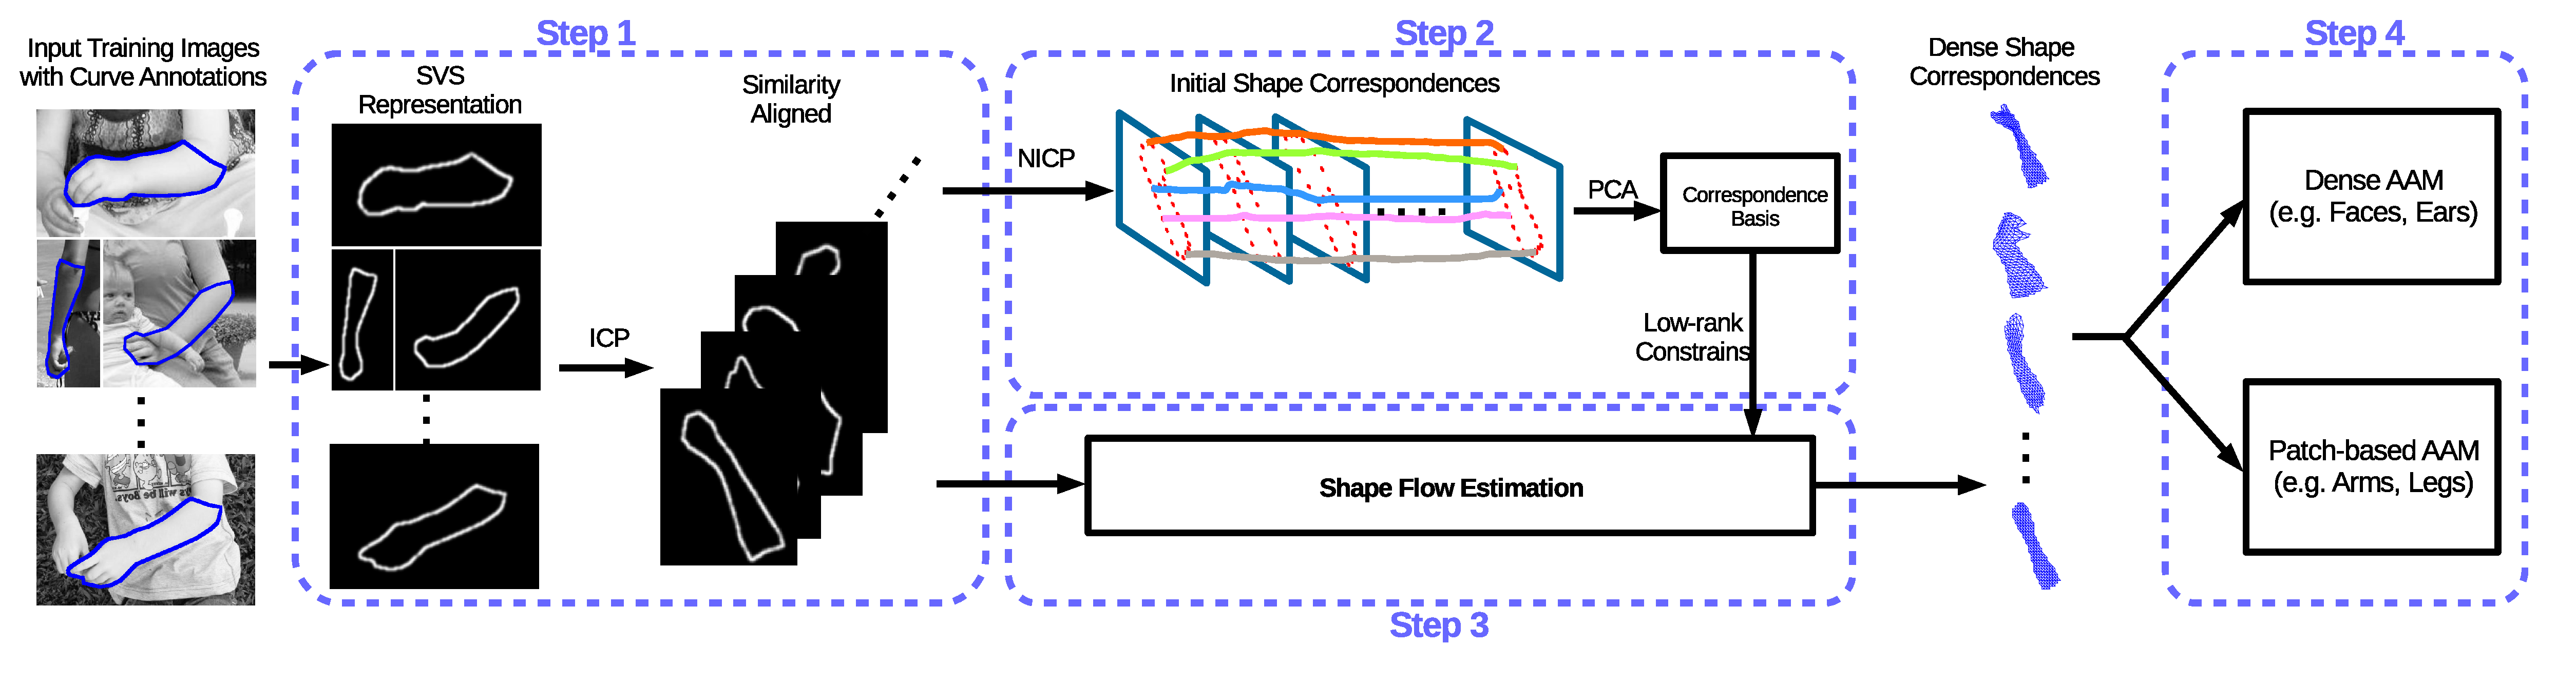
\includegraphics[width=\textwidth]{resources/architecture3}
    \caption{Schematic description of the proposed pipeline. Figure best viewed by zooming in.}
    \label{fig:archi}
\end{figure*}

\section{Constructing Deformable Models with Shape Flow}

% Deformable models are widely used for object detection, localization, recognition and tracking while training a deformable model with good generalisation requires tremendous amount of carefully annotated data, which is extremely time consuming. Even more, annotated data of a specific object category typically requires same numbers of landmarks for every training sample, making the annotation procedure significantly complex where corrext menual annotation of landmarks is impossible in various object classes e.g. ears.

% Despite the fact that that vast majority of existing methods are based on a sparse shape representation, dense shape representation reveals more nuanced structure in terms of [todo: explain].

We propose a novel framework for building deformable models that does not require any consistent set of annotated landmarks and is based on a dense shape representation. Our method only requires a set of point or curve line annotations that does not need to be consistent over different training samples. It combines the techniques of Non-rigid Iterative Closest Point (NICP) \cite{Amber2007}, multi-channel Support Vector Shape (SVS) \cite{Nguyen2013} representation and multi-image subspace flow \cite{Garg:2013hu} in an effective framework that has significant descriptive power.

The proposed pipeline is depicted in Figure~\ref{fig:archi}. It takes as input a set of training images of a particular object class, along with inconsistent point and/or curve line annotations.
As a first step, all the shape annotations are consistently represented using multichannel SVS.
The next step is the application of Iterative Closest Point (ICP) algorithm \cite{Besl1992} to achieve an initial simple alignment of the SVS images.
The multichannel similarity-aligned SVS images are then fed into a multi-image subspace flow estimation that establishes dense correspondences between all the shapes in the training set. In order for the flow estimation to be accurate and exploit the correlation among all training shapes, it utilises a correspondence basis built from sparse correspondences obtained by applying Nonrigid ICP on the annotated data. Finally, the dense correspondences yield by optical flow serve as automatically generated dense landmark annotations and are used to define a novel dense version of Active Appearance Models. The upcoming sections discuss each of the previous stages in further detail.

%two major modules. The first module handles inconsistent annotation set by converting to landmark independent shape discriminator. While the other module produces shape flow on object discriminators to generate dense flow transformations in shape space following by robust PCA\cite{?} to generate deformable model. In this section, we present the entire architectures, design decision and algorithms.
\subsection{Shape Representation Without Consistent Annotations}
\label{sec:svs}
%Ordinarily, construction of deformable model requires training data set having consistent number of landmarks. But unavoidable changes has to be made before applying same algorithm on diverse annotated data set.

In order to fully capture the variability among most deformable object shapes annotations, we use a representation based on Support Vector Shapes (SVS) \cite{Nguyen2013}. A SVS is a decision function trained on shapes using Support Vector Machines (SVMs) with Radial Basis Function (RBF) kernels. In this way, a shape is represented as a classifier function, which has several advantages: (a) the representation is completely general, \eg it can be applied to sparse landmark points, curves lines or a combination of the two and (b) it fuses inconsistent landmarks into consistent and directly comparable decision functions. Furthermore, this representations is also robust against noise, missing data and outliers \cite{Nguyen2013}.

In practice, we assume that all the training images correspond to the same object category and contain a set of inconsistent points and curve line annotations. All annotations are densely sampled to yield a set of annotated landmarks per image, with this set being different for every training image. Initially, negative points get randomly sampled around sparse landmarks while annotated landmarks are positive points. Since the number of positive points is far smaller that the number of negative ones, landmarks are assigned considerably larger weights so that $N_p \times W_p=N_n \times W_n$ where $N_p, N_n$ are the number of positive/negative samples and $W_p, W_n$ are their corresponding weights.

SVMs with RBF kernel function map any number of data points onto an infinite-dimensional space where positive and negative points are linearly separable, hence the classification boundary on 2D space represents the actual shape of the object. Note that the decision function for SVMs can be mathematically expressed as:
\begin{equation} \label{eq:decisionfunc}
    d(\bm{x})=\sum_i\alpha_i \, k(\bm{x}_i^*,\bm{x})
\end{equation}
where $\bm{x}_i^*$ are the so-called support vectors and \mbox{$k(\bm{x}, \bm{y}) = \exp\left(-\frac{\|\bm{x} -\bm{y}\|^2}{2 \sigma^2}\right)$} is the RBF kernel .

Figure \ref{fig:build_svs} shows an exemplar shape representation using SVS. As it can be observed, the final result does not drastically depend on the original number of annotated landmarks.


% \begin{figure}[b!]
%     \centering
%     \begin{subfigure}[b]{0.2\textwidth}
%             \includegraphics[width=\textwidth]{resources/landmark}
%         \caption{Spare landmarks}
%     \end{subfigure}
%     \qquad
%     \begin{subfigure}[b]{0.2\textwidth}
%             
\includegraphics[width=\textwidth]{resources/svs}
%         \caption{Decision function}
%         \label{fig:svs}
%     \end{subfigure}
%     \caption{Exemplar SVS shape representation. The decision function is trained on the set of sparse landmarks. In (b), brighter colour represents higher probability of a pixels belonging to the original shape.}
%     \label{fig:build_svs}
% \end{figure}

\begin{figure}[b!]
    \centering
    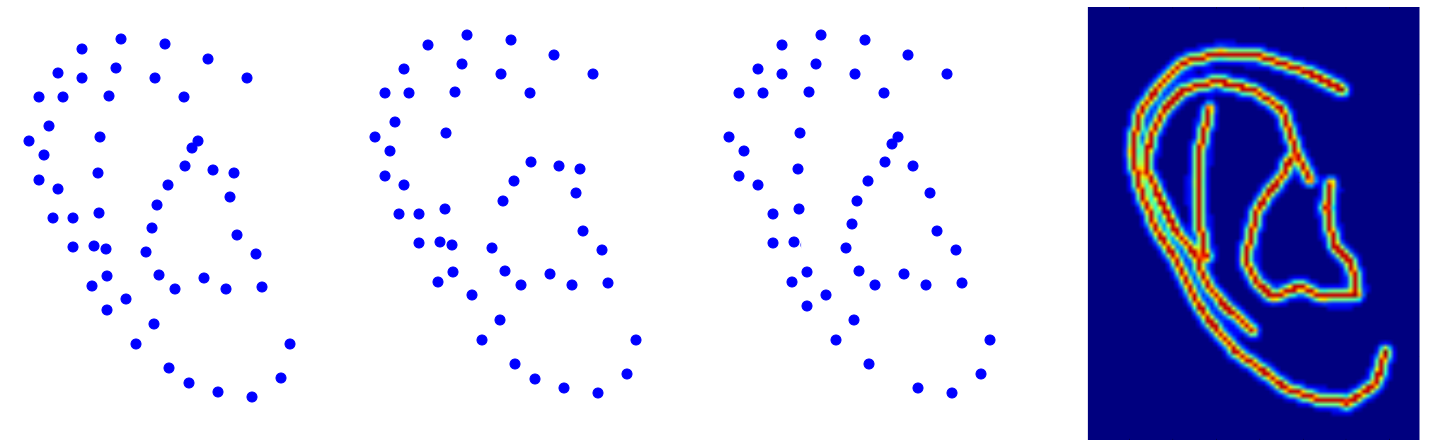
\includegraphics[width=0.4\textwidth]{resources/svs2}
    \caption{Exemplar SVS shape representation. A similar SVS image is obtained from different annotations of the same shape.}
    \label{fig:build_svs}
\end{figure}


After constructing the SVS representation for all images, the next step is to apply a simple similarity alignment over them. This is done because the goal here is to build a model capable of effectively representing non-rigid local shape deformations rather than global rotation, translation and scaling. The alignment is performed by using the Iterative Closest Point (ICP) algorithm \cite{Besl1992} on the annotated landmarks point cloud of the training images.


\subsection{Shape Correspondence Basis}

We consider the problem of dense correspondences across SVS images as a joint estimation of optical flow fields between a reference SVS image and every SVS image of the training dataset. The estimation of such a ``shape flow'' defines for every training SVS image a warping function that registers it with the reference SVS image. To establish the dense correspondences robustly, we are inspired by the idea of subspace constraints in the estimation of multiframe optical flow \cite{Garg:2013hu}.

Instead of the \emph{motion} basis used in multiframe optical flow formulation of \cite{Garg:2013hu}, we build a \emph{correspondence} basis that introduces constraints on how points of different shapes are matched to each other. Every pixel of the reference SVS image is matched to its corresponding position at every training SVS image and in this way defines a \emph{correspondence vector}. This vector consists of the 2D locations of the specific point in all SVS images. To form this vector, the training images are arranged in an arbitrary order. Similarly to the order of training samples when Principal Component Analysis (PCA) is applied, this order does not affect the result of our method and any re-ordering would produce exactly the same results.


Formally, let $F$ be the number of training SVS images and $n=1,\ldots,F$ be the training image index. Also, let $\boldsymbol{q}_1(n),\ldots,\boldsymbol{q}_R(n):
\{1,\ldots,F\} \rightarrow \R^2$ be the $R$ orthonormal elements of the correspondence basis, where $\boldsymbol{q}_i(n)$ is the displacement vector that matches the points of the reference SVS image with the points of the $n$-th training SVS image, according to the variation described from the $i$-th correspondence basis element. Note that the basis elements $\boldsymbol{q}_i(n)$ are independent from the point location. Note also that the number of basis elements is typically much smaller than the full dimensionality ($2 F$) of correspondence vectors, therefore this basis plays a role of dimensionality reduction.


In addition, let $\Omega \subset \R^2$ be the image domain of the SVS images and $\bx$ denote the point location. We denote the shape flow result as $\bm{u}_n(\bx):\Omega\times \{1,\ldots,F\}
\rightarrow \R^2$,  where $\bm{u}_n(\bx)$ is the displacement vector that matches the point $\bx$ of the reference SVS image with its corresponding location at the $n$-th training SVS image.

Using the constructed correspondence basis, the shape flow can be approximated as:
\begin{equation}\label{eq:LinTrajModel}
    \bm{u}_n(\bx) \approx
    \sum_{i=1}^R\bm{q}_i(n)\bm{v}_i(\bx) \,\, ,
\end{equation}
where $\bm{v}_i(\bx)$ is the weight that needs to be applied on the $i$-th correspondence basis element, in order to get the correspondence vector for the point location $\bm{x}$. In other words, the shape flow for every point $\bm{x}$ is described as a linear combination of basis elements that is controlled by the coefficients $\bm{v}_i(\bm{x})$.
The values of the $i$-th coefficient for all the points $\bm{v}_i(\bm{x})$ can be interpreted as an image defined on $\Omega$. Using the correspondence basis, the determination of the shape flow boils down to the determination of the set of coefficients $\bm{v}_i(\bm{x})$. The above representation of shape flow, constrains the correspondence vectors to lie on a subspace and, therefore, acts as a low-rank prior that enforces coherency of the shape registration result over the whole training dataset of shapes.


The next section describes the methodology of constructing the correspondence basis and estimating the shape flow robustly.

% For all dense transformations $\bm{u}_n(\bm{x}), n \in \{1,...,F\}$, where $F$ is number of data and $\bm{x}$ is vector of pixels, Principle Component Analysis (PCA) is performed on trajectory to obtain low rank trajectory basis:
% \begin{equation}
%     \begin{bmatrix}
%         \bm{u_1}(\bm{x}) \\
%         \vdots \\
%         \bm{u_F}(\bm{x})
%     \end{bmatrix}
%     =
%     \begin{bmatrix}
%         \bm{q_1}(1) & \cdots & \bm{q_R}(1) \\
%         \vdots      & \ddots & \vdots  \\
%         \bm{q_1}(F) & \cdots & \bm{q_R}(F)
%     \end{bmatrix}
%     \times
%     \begin{bmatrix}
%         \bm{v_1}(x) \\
%         \vdots \\
%         \bm{v_R}(x)
%     \end{bmatrix}
% \end{equation}
% where $\bm{q_i}(n)$ are low rank components with $R \ll 2F$ and $\bm{v_i}(x)$ weighted each component with dependencies on $x$. Simpler expression shown below:
% \begin{equation}
%     \bm{u}_n(\bm{x})=\sum_{i=1}^R\bm{q_i}(n)\bm{v_i}(x)+\bm{\varepsilon_n}(\bm{x})
% \end{equation}

\begin{figure}[t!]
        \centering
        \begin{tabular}{ccc}
        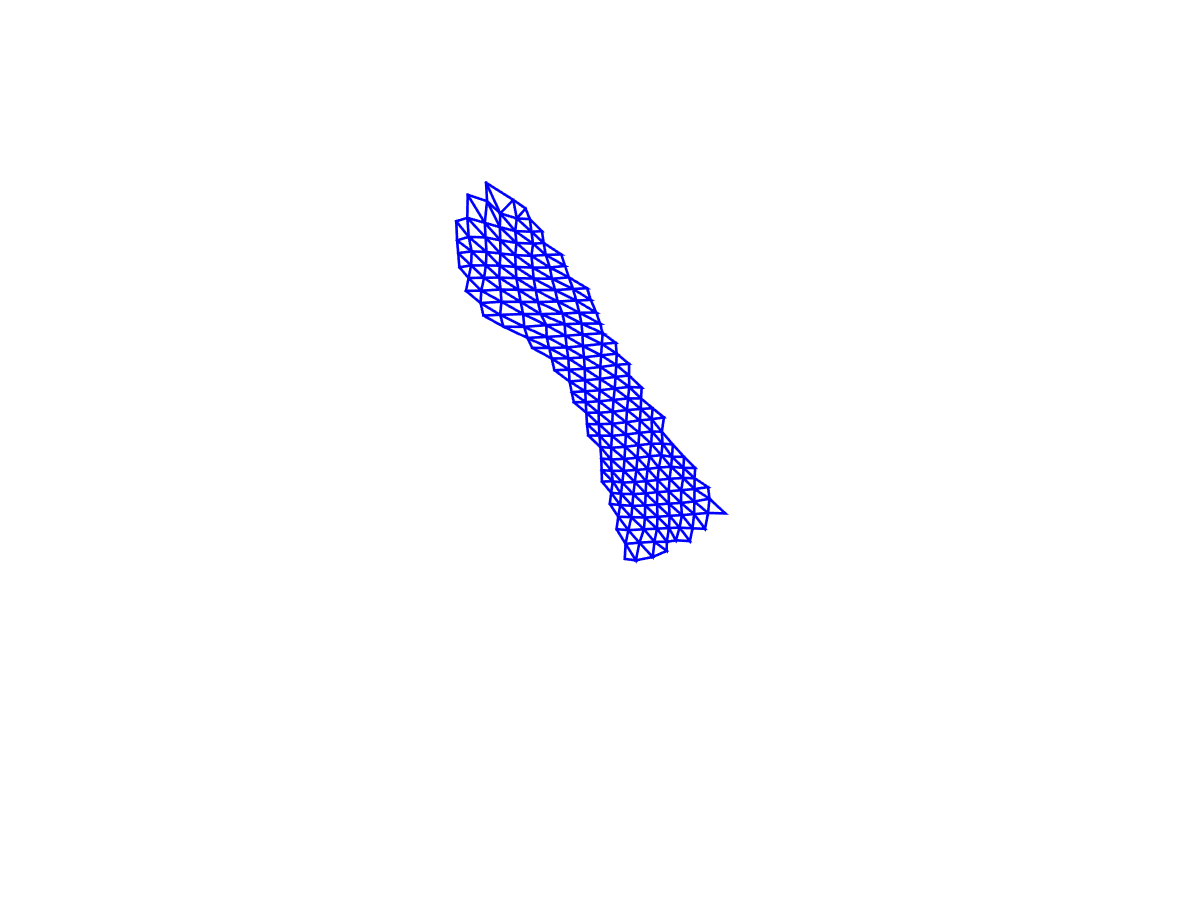
\includegraphics[trim=200 150 200 50,clip,width=.25\columnwidth]{resources/Fig_Flows/1}
        &
        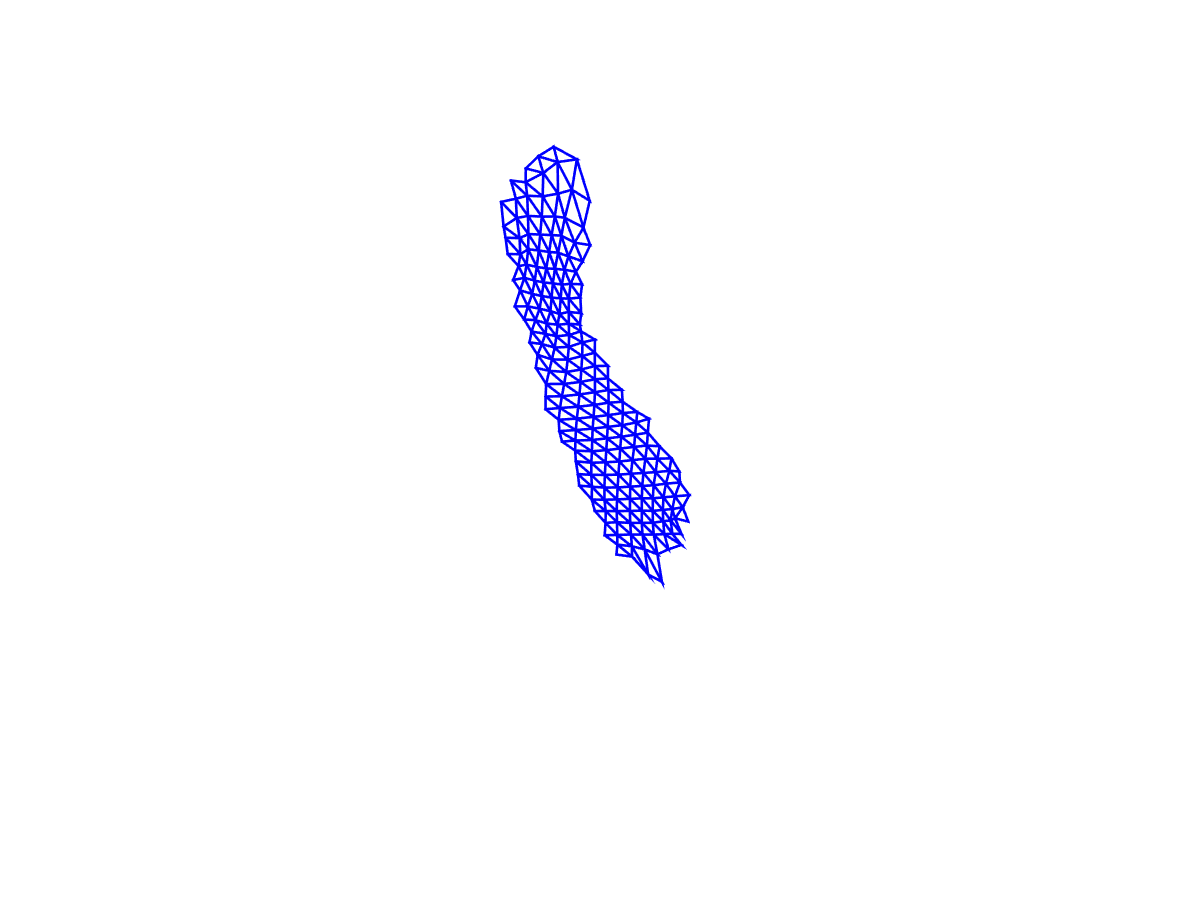
\includegraphics[trim=200 150 200 50,clip,width=.25\columnwidth]{resources/Fig_Flows/2}
        &
        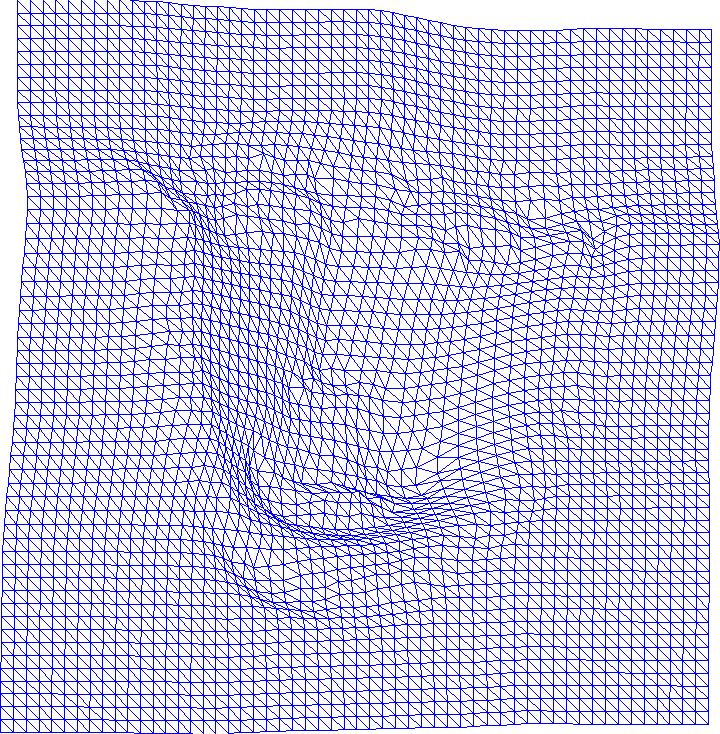
\includegraphics[trim=200 150 200 50,clip,width=.25\columnwidth]{resources/Fig_Flows/3}
        \\
        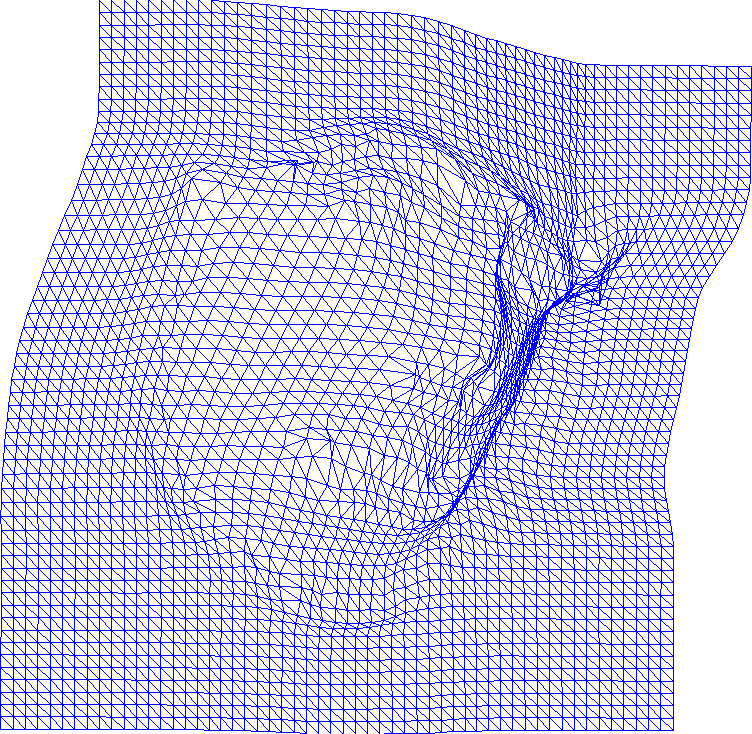
\includegraphics[trim=200 150 200 50,clip,width=.25\columnwidth]{resources/Fig_Flows/4}
        &
        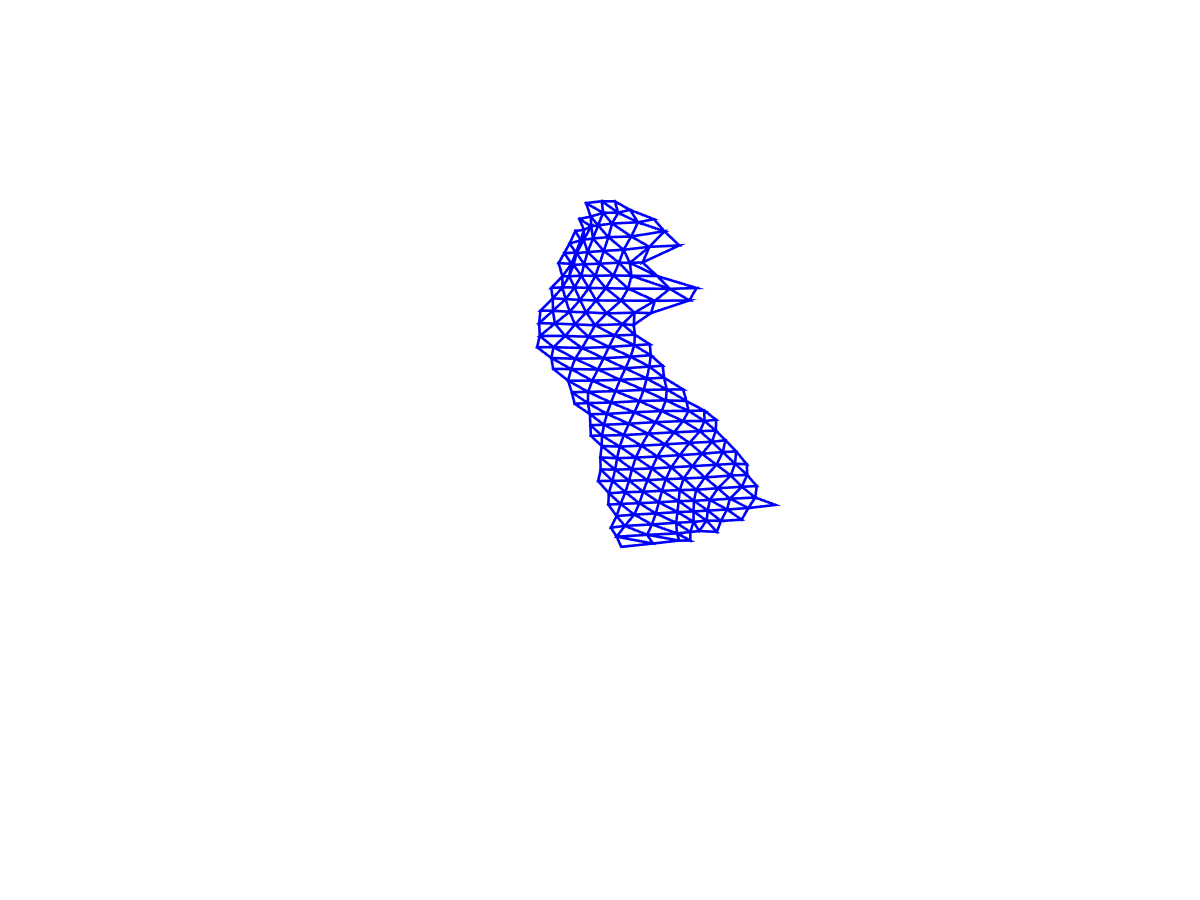
\includegraphics[trim=200 150 200 50,clip,width=.25\columnwidth]{resources/Fig_Flows/5}
        &
        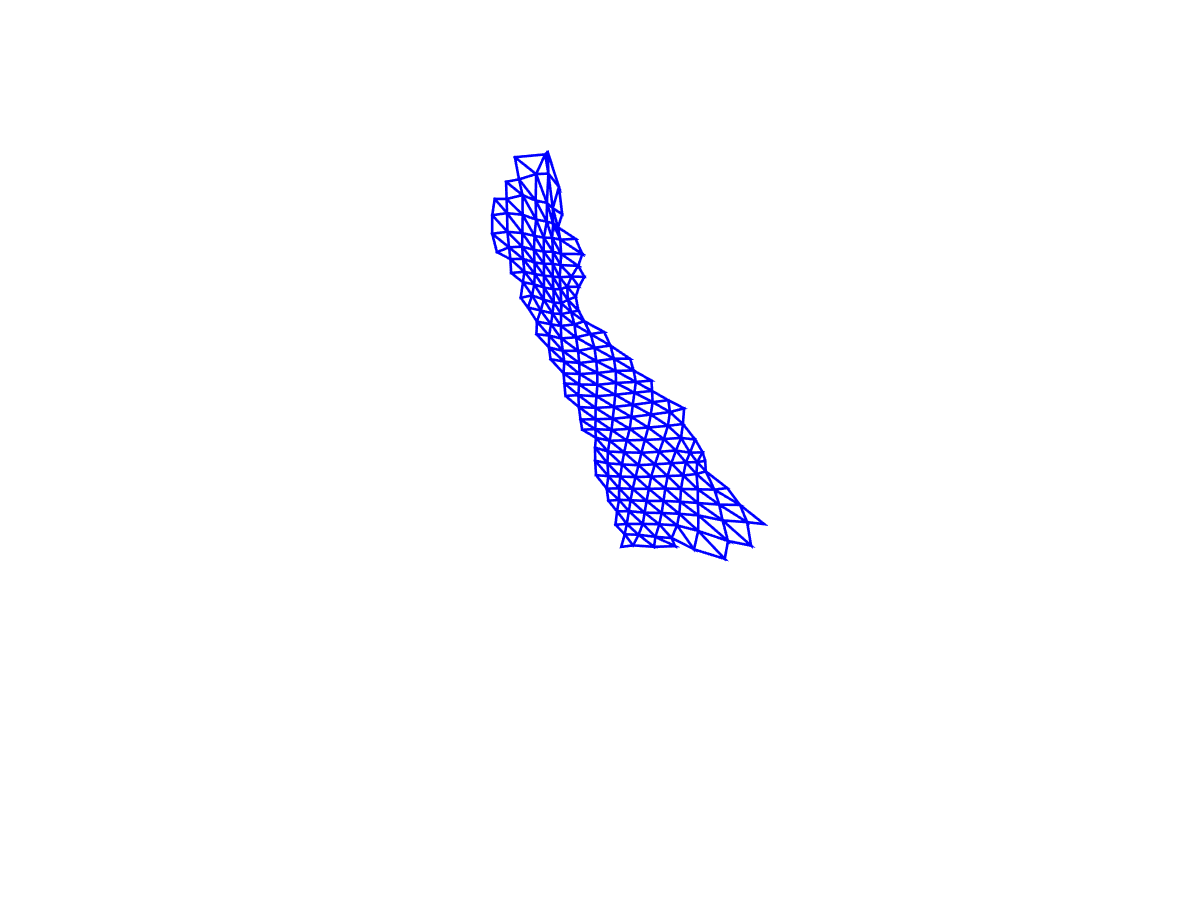
\includegraphics[trim=200 150 200 50,clip,width=.25\columnwidth]{resources/Fig_Flows/6}
        \end{tabular}
    \caption{Exemplar deformation fields for the left forearm, obtained using the proposed pipeline. Figure best viewed by zooming in.}
    \label{fig:deformationfield}
\end{figure}





% ---------------------------------------------------------------------------------------------------------------------------------------------------


\subsection{Shape Flow}
\label{sec:shapeflow}


Using the SVS functions built from training data, one of the main steps of our pipeline is to estimate dense correspondences between all these functions. We propose to perform this estimation simultaneously for all training data, by using the correspondence basis. This procedure, which we call \emph{shape flow}, builds upon robust methods for multiframe optical flow estimation \cite{Garg:2013hu}. However, optical flow estimation typically works based on the assumptions of brightness or colour constancy and motion smoothness, whereas in our setting the input training data correspond to shapes. For this reason, we propose to modify the formulation of \cite{Garg:2013hu} by using the correspondence basis that we introduced in conjunction with the SVS representation of shapes.


%
%In order to learn the such a subspace, we first transform the original annotation to point clouds. Then, we use NICP to align the previous point clouds with respect to a reference point cloud template. NICP iteratively deforms each point cloud until its points match the ones on the shape template and correspondences are established. However, because optical flow is a pixel-wise frame registration technique, we need to establish correspondences for all pixels on the reference frame rather than for sparse point clouds. To achieve this, we apply Thin Plate Spline (TPS) \cite{Bookstein1989} to find correspondences for all pixels in the reference frame given the point cloud correspondences provided by the previous NICP stage. Once dense correspondences have been established among all pixels, the so-called correspondence subspace is obtained by performing PCA the trajectory of all pixels. Note that incorporating the previous subspace as a low rank constrained in optical flow is consistent with its assumption of smooth motion.



\subsubsection{Non-rigid ICP and Correspondence Basis Creation} \label{sec:trabasis}



To effectively build the correspondence basis, we first transform the original annotations to sparse point clouds. Then, we apply Non-rigid Iterative Closest Point (NICP)\cite{Amber2007} between the point cloud of annotations in the reference shape and the one of every shape of the training set. NICP iteratively deforms the cloud of points of every shape to match the points of the reference shape. This yields an initial estimation of the correspondence vectors on the sparse locations of annotated landmarks on the reference shape. To make this correspondence vectors estimation dense (i.e.~for every pixel of the reference SVS image), we apply Thin-Plate Splines (TPS)\cite{Bookstein1989} interpolation. Finally, the correspondence basis is found by applying PCA on the result of TPS interpolation and keeping only the first $R$ principal components.




%
%
%Since optical flow pixel-wise frame registration, the trajectory basis build should also match the dimension, which is dense on shapes with trajectory length depends on number of training data. With correspondences produced after applying NICP, Thin-Plate Spline (TPS)\cite{Bookstein1989} transformations are utilized to warp every shape planes to template plane thereby generates an implicit dense shape registering. For all dense transformations $\bm{u}_n(\bm{x}), n \in \{1,...,F\}$, where $F$ is number of data and $\bm{x}$ is vector of pixels, Principle Component Analysis (PCA) is performed on trajectory to obtain low rank trajectory basis:
%\begin{equation}
%    \begin{bmatrix}
%        \bm{u_1}(\bm{x}) \\
%        \vdots \\
%        \bm{u_F}(\bm{x})
%    \end{bmatrix}
%    =
%    \begin{bmatrix}
%        \bm{q_1}(1) & \cdots & \bm{q_R}(1) \\
%        \vdots      & \ddots & \vdots  \\
%        \bm{q_1}(F) & \cdots & \bm{q_R}(F)
%    \end{bmatrix}
%    \times
%    \begin{bmatrix}
%        \bm{v_1}(x) \\
%        \vdots \\
%        \bm{v_R}(x)
%    \end{bmatrix}
%\end{equation}
%where $\bm{q_i}(n)$ are low rank components with $R \ll 2F$ and $\bm{v_i}(x)$ weighted each component with dependencies on $x$. Simpler expression shown below:
%\begin{equation}
%    \bm{u}_n(\bm{x})=\sum_{i=1}^R\bm{q_i}(n)\bm{v_i}(\bm{x})+\bm{\varepsilon_n}(\bm{x})
%\end{equation}
%Although optical flow on shapes made under the assumption that objects motion are smooth, the low rank constrain on trajectory basis recovered the hypothesis.

% \begin{figure}[t!]
%         \centering
%         \begin{tabular}{cccccccc}
%         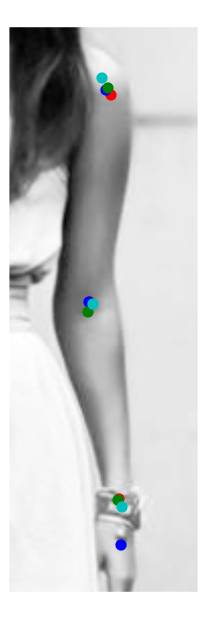
\includegraphics[trim=200 150 200 50,clip,width=.1\columnwidth]{resources/Fig_Variance/image_0}
%         &
%         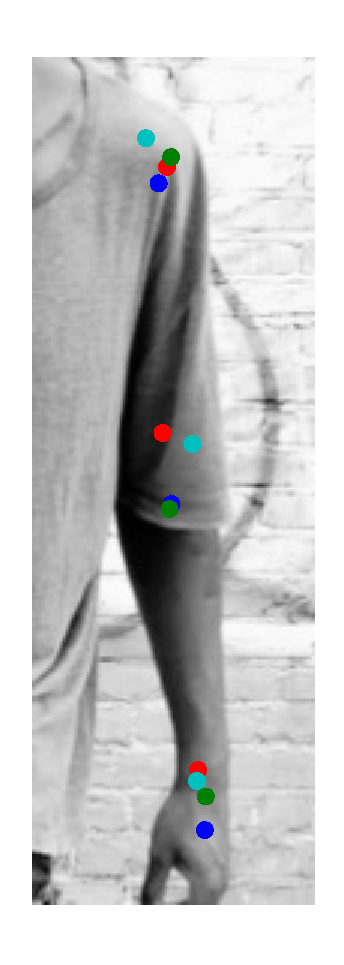
\includegraphics[trim=200 150 200 50,clip,width=.1\columnwidth]{resources/Fig_Variance/image_1}
%         &
%         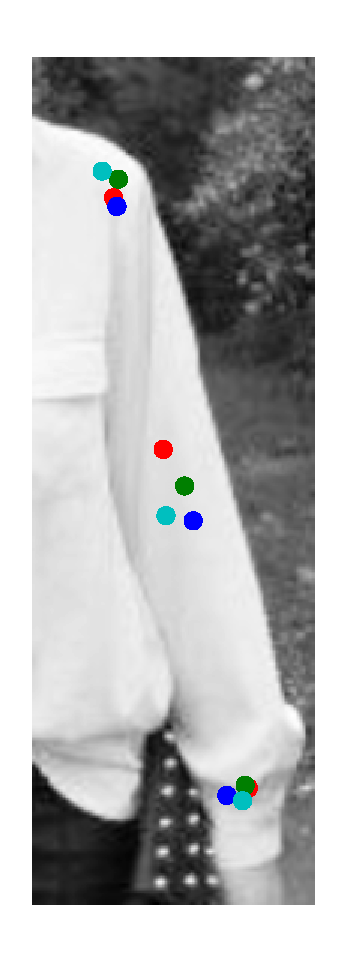
\includegraphics[trim=200 150 200 50,clip,width=.1\columnwidth]{resources/Fig_Variance/image_2}
%         &
%         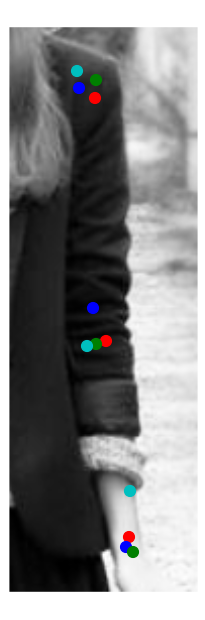
\includegraphics[trim=200 150 200 50,clip,width=.1\columnwidth]{resources/Fig_Variance/image_3}
%         &
%         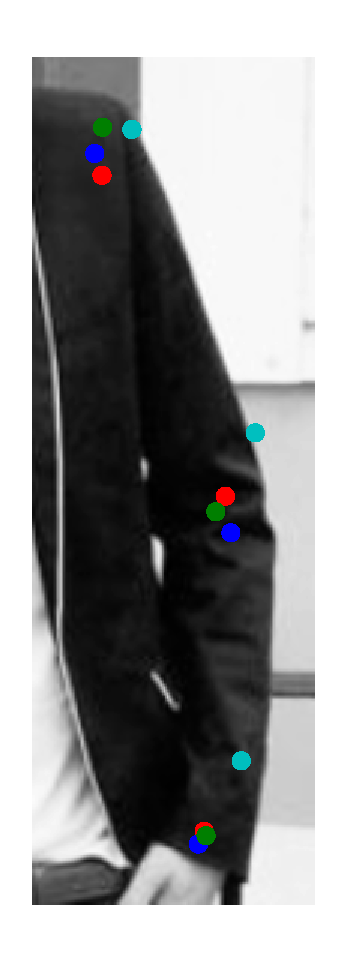
\includegraphics[trim=200 150 200 50,clip,width=.1\columnwidth]{resources/Fig_Variance/image_4}
%         &
%         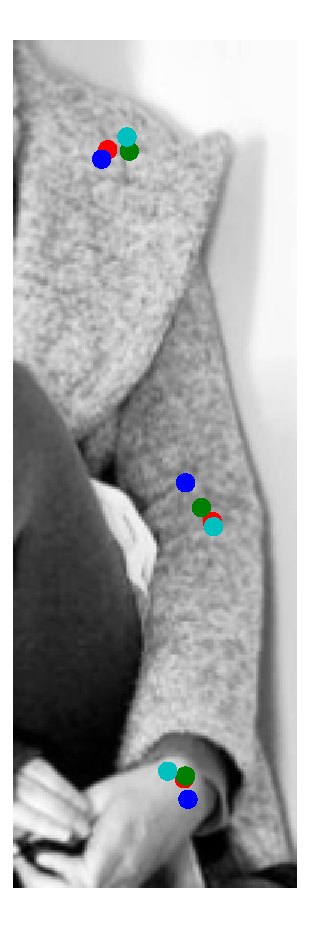
\includegraphics[trim=200 150 200 50,clip,width=.1\columnwidth]{resources/Fig_Variance/image_5}
%         &
%         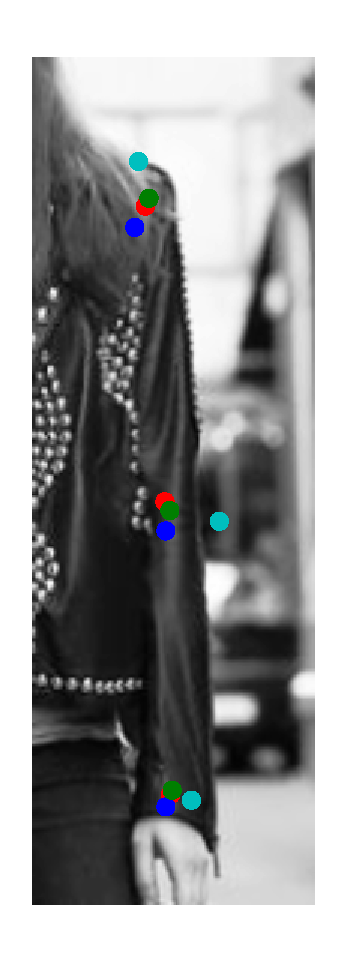
\includegraphics[trim=200 150 200 50,clip,width=.1\columnwidth]{resources/Fig_Variance/image_6}
%         &
%         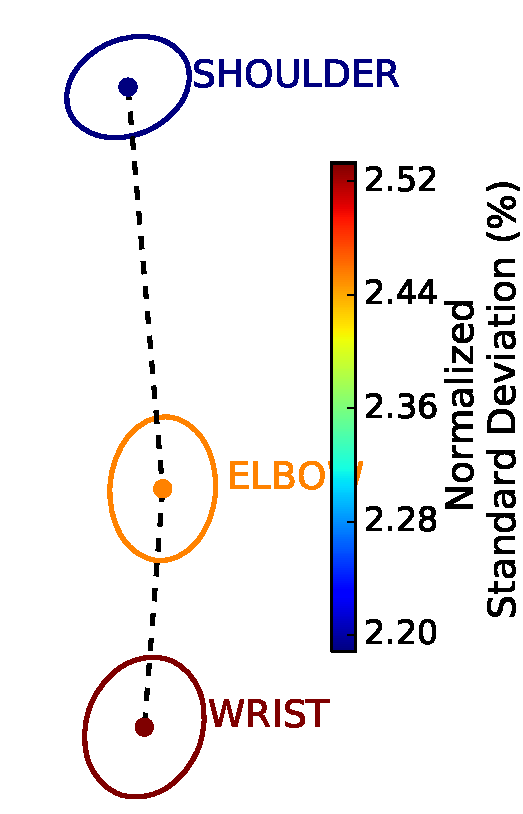
\includegraphics[trim=200 150 200 50,clip,width=.1\columnwidth]{resources/Fig_Variance/variances}
%         \end{tabular}
%     \caption{Variances}
%     \label{fig:variances}
% \end{figure}

\begin{figure}[t!]
    \centering
    \begin{subfigure}[b]{0.05\textwidth}
            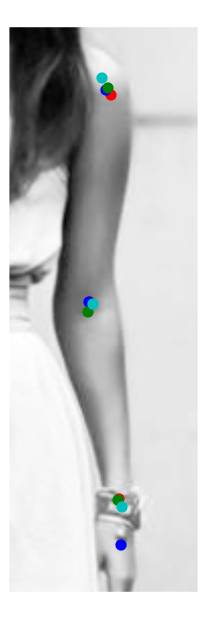
\includegraphics[width=\textwidth]{resources/Fig_Variance/image_0}
    \end{subfigure}
    \hfill
    \begin{subfigure}[b]{0.05\textwidth}
            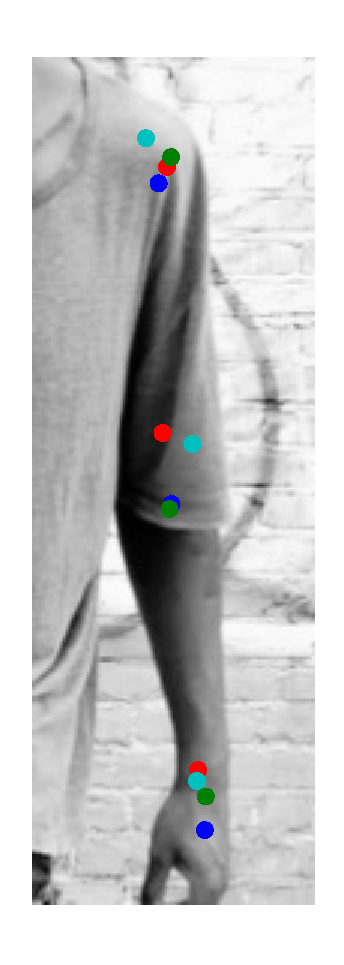
\includegraphics[width=\textwidth]{resources/Fig_Variance/image_1}
    \end{subfigure}
  	\hfill
    \begin{subfigure}[b]{0.05\textwidth}
            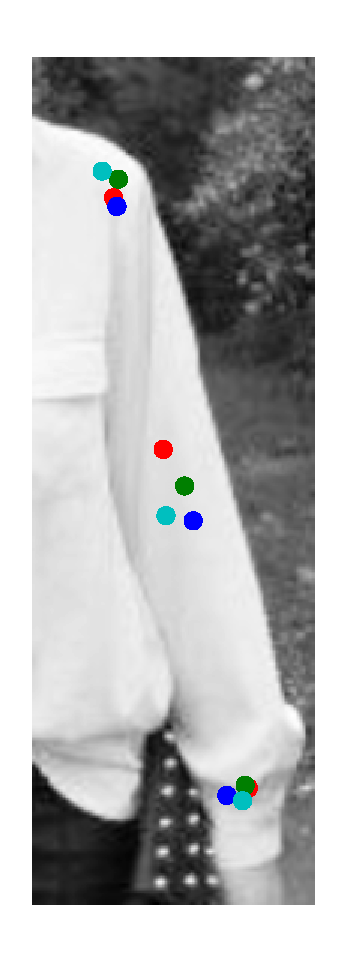
\includegraphics[width=\textwidth]{resources/Fig_Variance/image_2}
    \end{subfigure}
    \hfill
    \begin{subfigure}[b]{0.05\textwidth}
            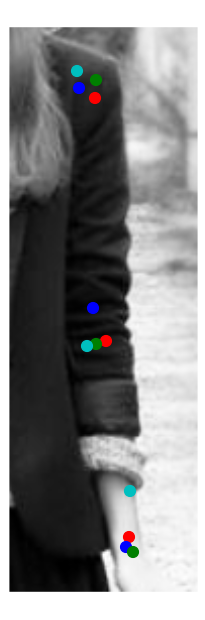
\includegraphics[width=\textwidth]{resources/Fig_Variance/image_3}
    \end{subfigure}
    \hfill
    \begin{subfigure}[b]{0.05\textwidth}
            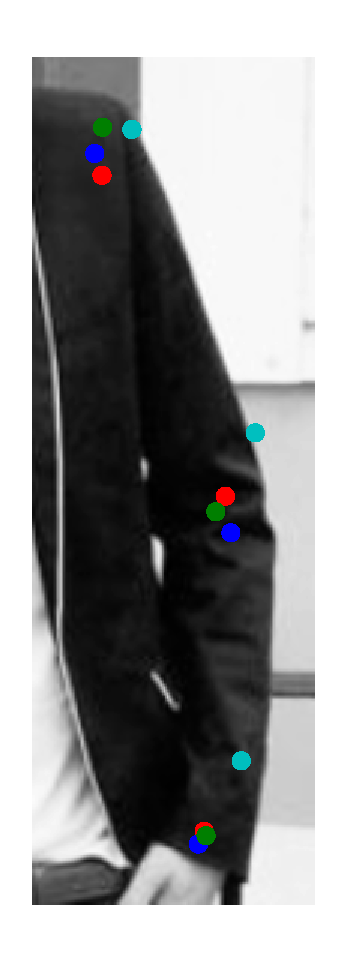
\includegraphics[width=\textwidth]{resources/Fig_Variance/image_4}
    \end{subfigure}
  	\hfill
    \begin{subfigure}[b]{0.05\textwidth}
            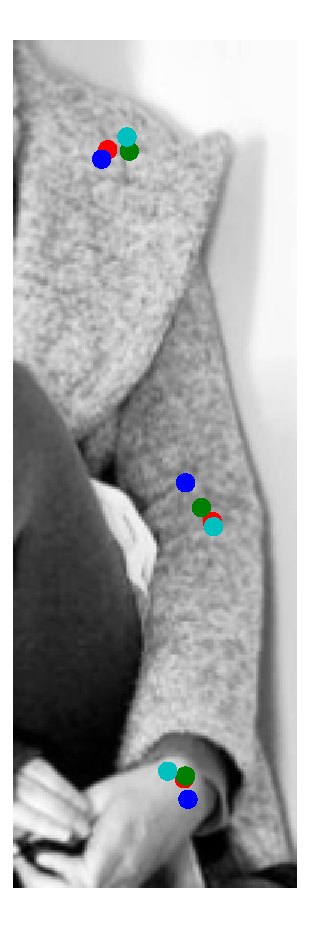
\includegraphics[width=\textwidth]{resources/Fig_Variance/image_5}
    \end{subfigure}
    \hfill
    \begin{subfigure}[b]{0.05\textwidth}
            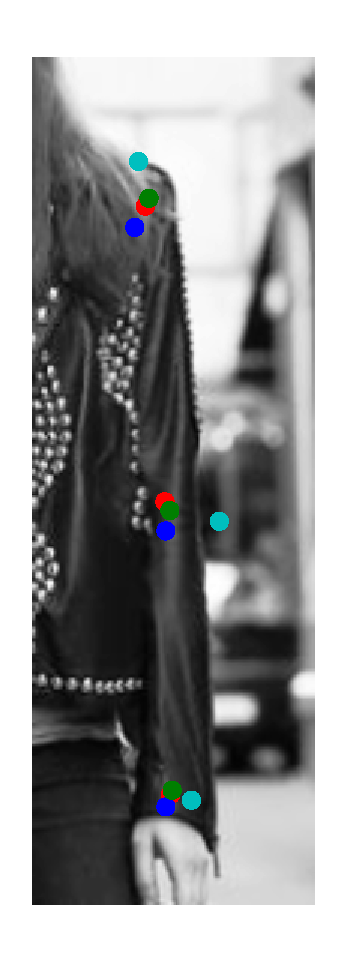
\includegraphics[width=\textwidth]{resources/Fig_Variance/image_6}
    \end{subfigure}
    \hfill
    \begin{subfigure}[b]{0.08\textwidth}
            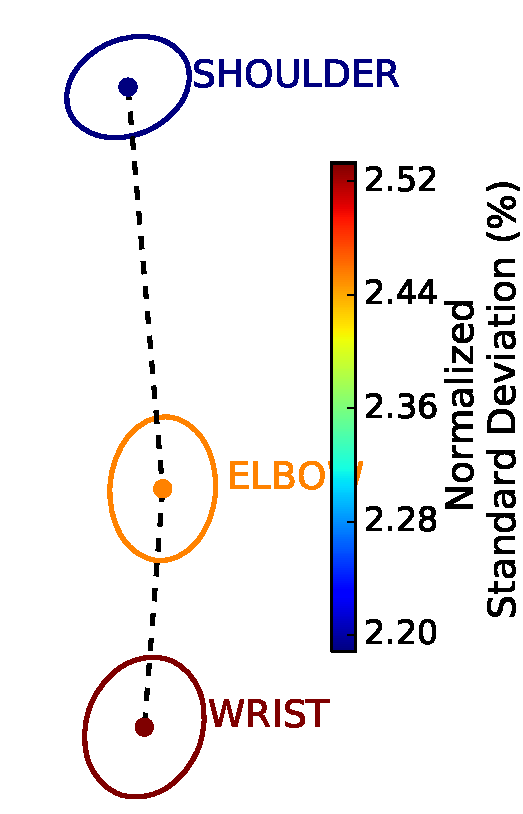
\includegraphics[width=\textwidth]{resources/Fig_Variance/variances}
    \end{subfigure}
    \caption{Variance.}
    \label{fig:variance}
\end{figure}




\subsubsection{Variational Shape Flow Estimation}%{Multi-image Subspace Flow}
\label{varshapeflow}

Following \cite{Garg:2013hu}, we propose to estimate the shape flow over all training SVS images $\bm{d}_n(\bx)$ by minimizing the following energy:
\begin{align}
E_{sf} & =\alpha
\int_{\Omega}\sum_{n=1}^F \|\bm{d}_n(\bx+\bm{u}_n(x))-\bm{d}_0(x)\| \ud \bx \label{eq:costfunc}\\
    &+ \beta \int_{\Omega}\sum_{n=1}^F\|\bm{u}_n(\bx)-\sum_{i=1}^R\bm{q}_i(n)\bm{v}_i(\bx)\|^2 \ud \bx \label{eq:lowrank}\\
    &+
\int_\Omega  \sum_{i=1}^R \,\, \left \|    \nabla \bm{v}_i(\bx)    \right \|  \,\ud \bx \label{eq:TVterm}
\end{align}
This energy consists of two sets of unknown shape flows that are relatively close to each other: (i) $\bm{u}_n(x)$ which tries to explain the data from the input SVS images, and (ii) the shape flow determined by the correspondence basis coefficients $\bm{v}_i(\bx)$ that are spatially regularised and enforce a low-rank prior. We minimize this energy jointly with respect to $\bm{u}_n(\bx)$ and $\bm{v}_i(\bx)$. The positive parameters $\alpha$ and $\beta$ weigh the balance between the terms of the energy.

The \textbf{first term} of the above energy \eqref{eq:costfunc} is a data attachment term
that uses the robust $\Lone$-norm.  It is based on the assumption that the values of the reference SVS image $\bm{d}_0(\bx)$ at every pixel $\bx$ are preserved at its corresponding locations on all training SVS images $\bm{d}_n(\bx)$. The use of an $\Lone$-norm improves the robustness of the method since it allows deviations from this assumption, which might occur in practice.
The \textbf{second term} of the energy \eqref{eq:lowrank} penalizes the difference between the two sets  of shape flows and acts as a coupling term between them.
The \textbf{third term} of the energy \eqref{eq:TVterm} corresponds to the spatial Total Variation regularization \cite{rudin92} of
the correspondence basis coefficients $\bm{v}_i(\bx)$.
This term penalizes spatial oscillations of each coefficient caused by distortions of the SVS images but not strong discontinuities that are desirable in the borders of different object regions. In addition, this term allows to fill in information into regions where the shape information in the SVS images is missing, due to e.g.~regions with no annotations.

We implement the minimization of the energy $E_{sf}$ by using the optimization algorithm described in \cite{Garg:2013hu}. In every coarse-to-fine and warping iteration, we use an initialization that comes from the previous iteration and for the very beginning, we initialize with the shape flow result of the TPS interpolation described in Sec.~\ref{sec:trabasis}. We approximate the data term \eqref{eq:costfunc} by linearizing the SVS images around the initialization. After that, the energy becomes convex and we optimize it using alternating optimization w.r.t.~$\bm{v}_i(\bx)$ and $\bm{u}_n(\bx)$. The minimization w.r.t.~
$\bm{v}_i(\bx)$ is decoupled for every coefficient $i$ and corresponds to Rudin-Osher-Fatemi Total Variation denoising \cite{rudin92}, which we solve efficiently by applying the first order primal-dual algorithm of \cite{Chambolle:Pock:JMIV2011}. The minimization w.r.t.~
$\bm{u}_n(x)$ is decoupled for every pixel $\bx$ and every shape index $i$. This minimization is also implemented by applying the efficient primal-dual algorithm of \cite{Chambolle:Pock:JMIV2011}.



Figure~\ref{fig:deformationfield} shows some examples of deformation fields derived from the estimated shape flow computed by the aforementioned method. These results correspond to exemplar training shapes in the case of a face dataset.


%
%
%To register all decision functions to temp`late shape, decision function $d_i(\bm{x}), i \in {1,...,F}$ are grouped into one sequence before applying flow algorithm. The objective cost function we would like to minimise is:
%\begin{align}
%    \operatorname*{arg\,min}_{\bm{u}_n(\bm{x}), \bm{v}}&=\alpha \int_{\Omega}\sum_{n=1}^F|\bm{d_n}(x+\bm{u}_n(x))-\bm{d_0}(x)\| dx  \label{eq:costfunc}\\
%    &+ \beta \int_{\Omega}\sum_{n=1}^F\|\bm{u}_n(x)-\sum_{i=1}^R\bm{q_i}(n)\bm{v_i}(x)\|^2 dx \label{eq:lowrank}\\
%    &+ \sum[\bm{TV}(Qv)]
%\end{align}
%where $d_n(x)$ is the decision function from~\eqref{eq:decisionfunc}, which returns possibilities of given coordinate classified as shape component where coordinates are from set $\Omega \in \Re^2$. $TV(Qv)$ is total variation as regularization on low rank subspace, $Q$ is trajectory basis and $v^T.L.v$ is low rank spacial constrains.
%
%Term~\eqref{eq:costfunc} state the shape constancy where points having similar classification probability are from same object.
%Part~\eqref{eq:lowrank} applies constrain on low rank trajectory basis states in section~\ref{sec:trabasis}.
%The objective cost function has two free parameters $u$ and $v$, so we perform alternating minimisation. The equation can be solved using a thresholding scheme after linearisation of image functions. The minimisation can be speed up by paralleling the minimisation for every spatial-temporal point $(x;n), x \in \Omega, n \in \{1,...F\}$ independently.
%
%
%
%
%
%
%After solving the equation, $\bm{u}_n(\bm{x}), x \in \Omega$ gives a group of deformation fields that registering every decision functions in the shape sequence to reference frame e.g. $\bm{u_1}(\bm{x})$ registers decision function $\bm{d_1}(\bm{x})$ to the reference frame. Figure~\ref{fig:deformationfield} demonstrates deformation fields that warps from reference frame where there is no deformation.

% \begin{figure}[h!]
%     \centering
%         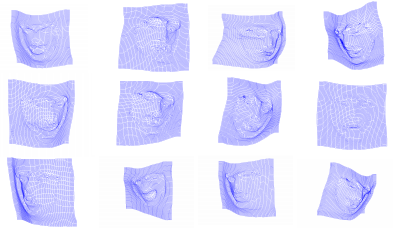
\includegraphics[width=0.5\textwidth]{resources/df}
%     \caption{Deformation field built}
%     \label{fig:deformationfield}
% \end{figure}



% Applying PCA on deformations trains dense deformable shape model:
% \begin{equation*}
%     \bm{s_p}=\bm{\bar{s}} + \bm{U}_s\bm{p}
% \end{equation*}
% where $\bm{s_p}$ is deformed shape instance. $\bm{\bar{s}}$ is mean shape and $\bm{U}_s\bm{p}$ are eigenvectors with corresponding parameters $p$. Figure~\ref{fig:models} shows an instance of deformed shape and appearance model.
% \begin{figure}[h!]
%     \centering
%     \begin{subfigure}[b]{0.22\textwidth}
%             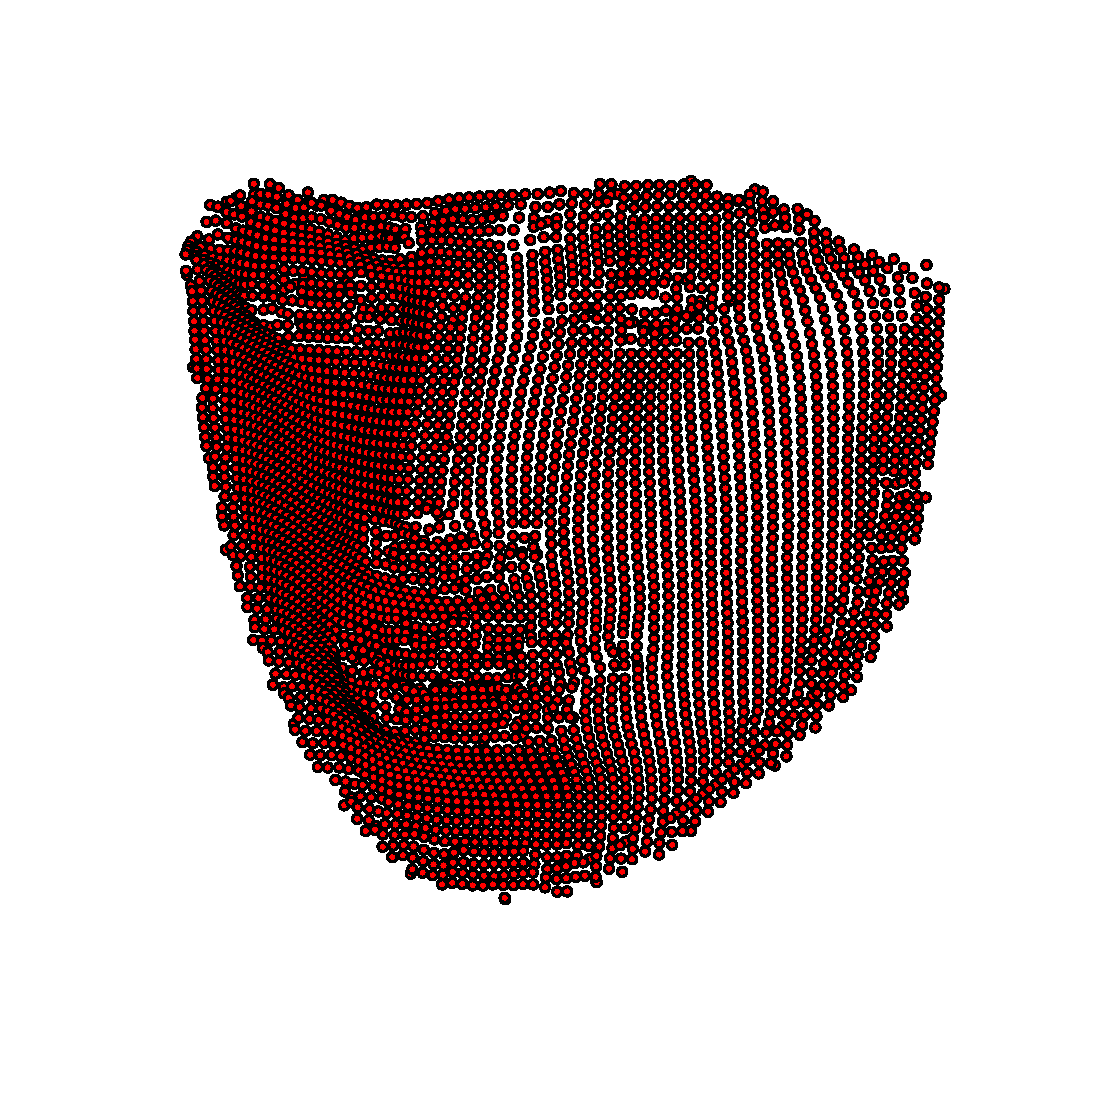
\includegraphics[width=\textwidth]{resources/Fig_dAAM/of_shape}
%     \end{subfigure}
%   	\hfill
%     \begin{subfigure}[b]{0.22\textwidth}
%             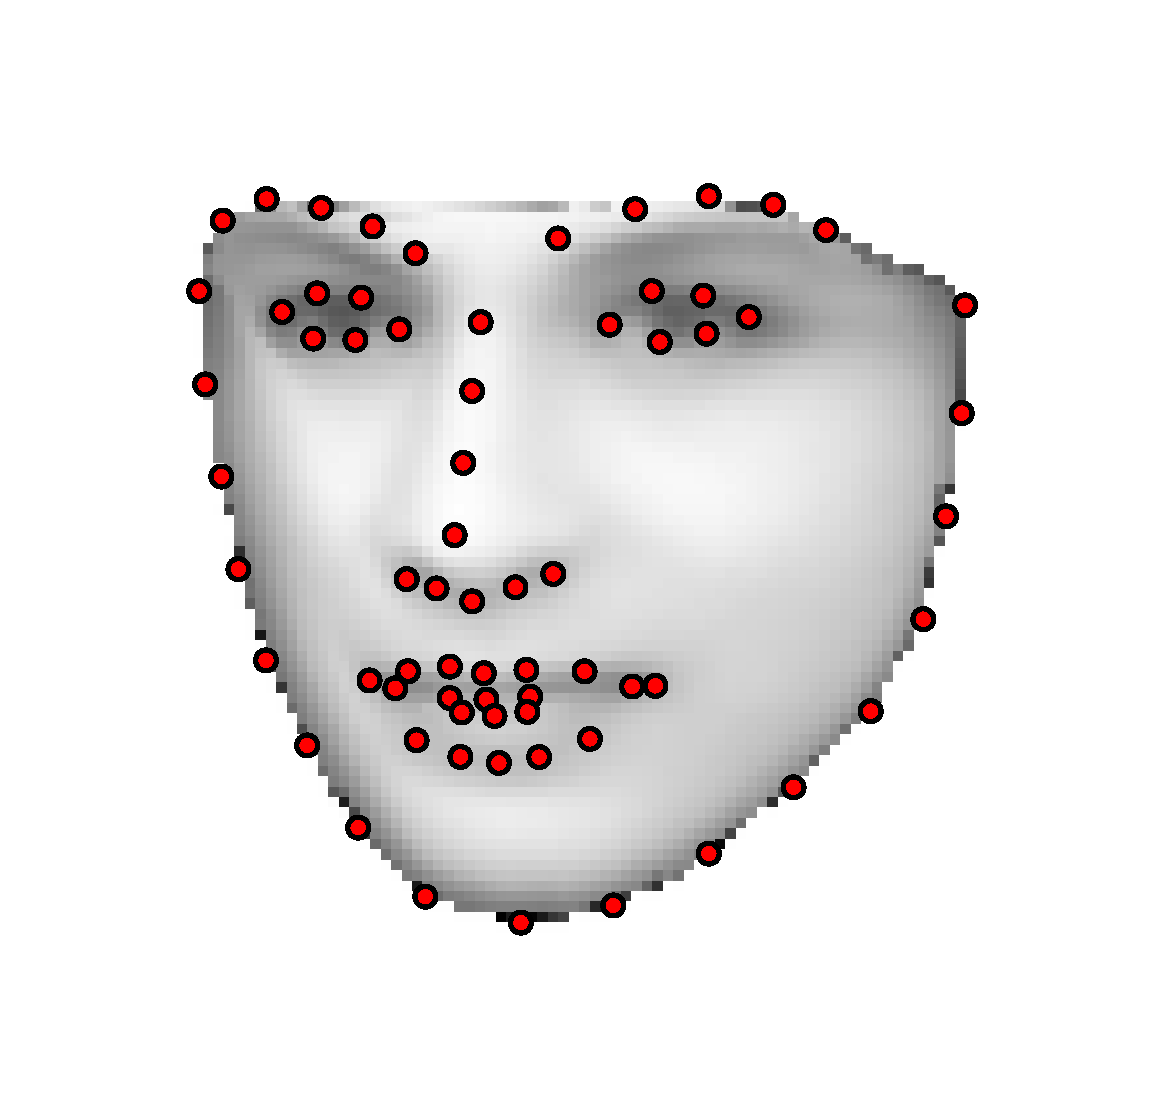
\includegraphics[width=\textwidth]{resources/Fig_dAAM/of_app}
%     \end{subfigure}
%     \caption{Dense Deformable Model}
%     \label{fig:models}
% \end{figure}

% \begin{figure}[h!]
%     \centering
%     \begin{subfigure}[b]{0.22\textwidth}
%             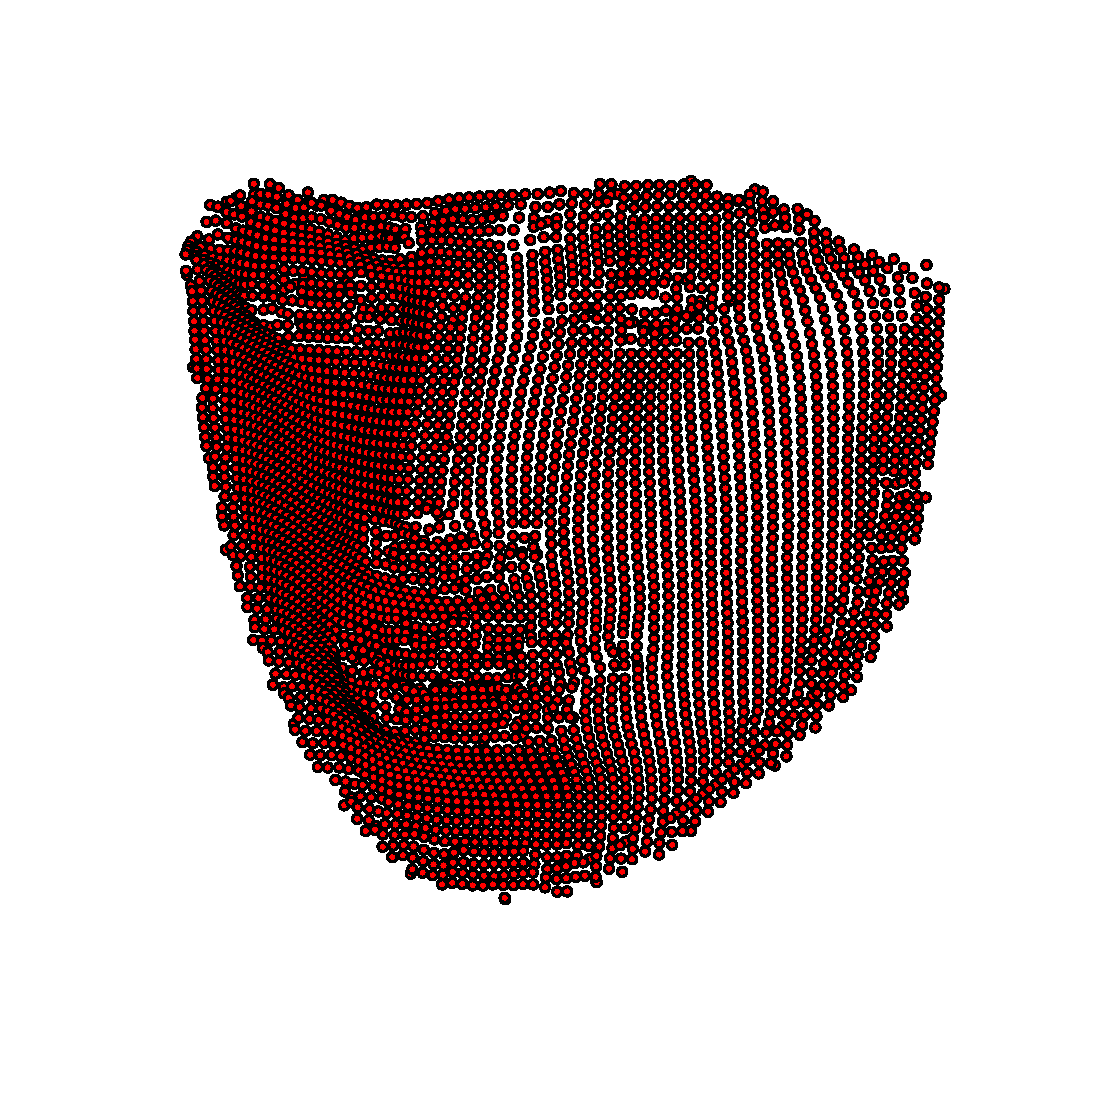
\includegraphics[width=\textwidth]{resources/Fig_dAAM/of_shape}
%     \end{subfigure}
%   	\hfill
%     \begin{subfigure}[b]{0.22\textwidth}
%             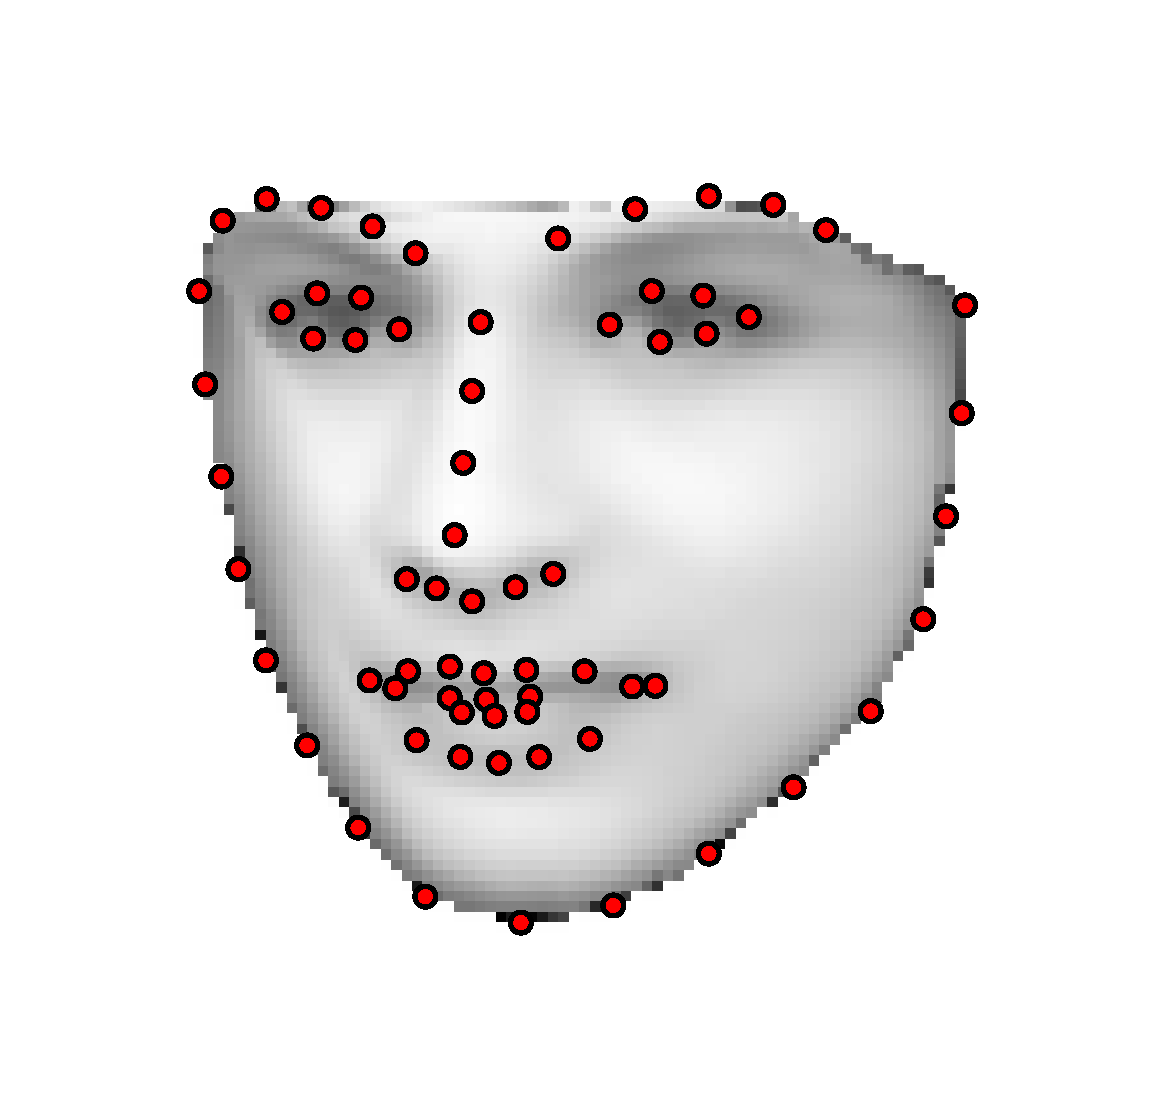
\includegraphics[width=\textwidth]{resources/Fig_dAAM/of_app}
%     \end{subfigure}
%     \caption{Dense Deformable Model}
%     \label{fig:models}
% \end{figure}

\subsection{Dense Active Appearance Models}

The deformation fields obtained from section \ref{sec:shapeflow} can be effectively used to learn a naturally dense version of Active Appearance Models \cite{Cootes2001, Matthews2004}. Because all deformation fields contain the same number of pixels (the same as on the reference frame) the spatial positions $\bm{x}_i=(x_i, y_i)$ of these pixels can be treated as point landmarks and the deformation field themselves as dense annotations of the object's shape. Consequently, building a dense shape model reduces to normalizing these dense annotations with respect to a global similarity transform (typically using Procrustes Analysis) and applying Principal Component Analysis (PCA). The resulting shape model can be mathematically expressed as:
\begin{equation}
    \begin{aligned}
        \bm{s} & = \bm{\bar{s}} + \bm{S} \bm{p}
    \end{aligned}
    \label{eq:shape_model}
\end{equation}
where $\bm{\bar{s}}$ is mean shape and $\bm{S}$ and $\bm{p}$ are the shape bases and shape parameters respectively.

On the other hand, the texture model associated to the previous set of densified shapes can be easily obtained by warping all image onto the reference frame, making explicit use of the one-to-one correspondence between pixels on the reference frame and on the deformation fields. Once the images have been warped, the texture model is obtained by applying PCA on the warped images. The texture model is mathematically defined by the following expression:
\begin{equation}
    \begin{aligned}
        \bm{t} = \bm{\bar{t}} + \bm{T} \bm{c}
    \end{aligned}
	\label{eq:tex_model}
\end{equation}
where $\bm{t}$ is the mean texture, and $\bm{T}$ and $\bm{c}$ are the texture bases and texture parameters respectively.

Note that, both shape and texture models are directly related through the established one-to-one correspondence between dense landmarks and pixels on the reference frame. Therefore, in clear contrast to classic AAMs formulations \cite{Cootes2001, Matthews2004}, in our dense formulation no motion model (piece-wise affine, thin-plates splines \cite{Bookstein1989}) is required to relate the previous shape and texture models . As noted in other works \cite{Amberg2009, Tzimiropoulos2014}, this has the advantage that all efficient compositional gradient descent algorithms for fitting AAMs \cite{Papandreou2008, Matthews2004, Amberg2009, Tzimiropoulos2013, Alabort2014} become exact under our formulation.

This shape flow-based dense AAM formulation provides an exceptionally effective modeling and fitting for various objects, such as ears and faces, whose appearance has characteristic structures spread all over the object region (even if these structures cannot be consistently annotated). Therefore, what has been described so far completes our proposed approach in training and fitting deformable models of this type of objects.

However, there exist other challenging object types, such as forearms, legs and full body, that not only cannot be consistently annotated with landmarks, but also whose appearance is informative almost entirely on the object outline and not in the interior object region. This is due to the hugely varying texture of these objects (e.g.~colors and patterns of clothes) that is typically totally unrelated to their shape. For these cases, we propose to add some additional steps on our methodology. More specifically, we propose to focus on the dense correspondences solely on the object outline, utilize them to automatically estimate highly-accurate object skeleton landmarks and then adopt a parts-based deformable modeling. These steps will be described in the next section.


\subsection{Outline-based Deformable Modeling}

As already mentioned, for estimating body pose and modeling other object types with similar challenges, we propose to only consider the established correspondences on the object outline.

Based on the proposed shape flow framework, we develop a methodology for robust automatic landmarking of the object outline. This allows a small initial training set that is manually annotated without consistent landmarks to be expanded to a much larger training set in an automatic way. In more detail, regarding the manually annotated images, for which SVS functions have been constructed, the outline correspondences are yielded by evaluating the estimated shape flow on the object outline of the reference image. To expand the training set to images without any annotations, we fit the trained dense AAM on these images and then only consider the deformed positions of the dense landmarks that correspond to the object outline on the mean shape.

Having reliable object outline annotations on a large training set, we appropriately fuse their information to infer consistent landmarks on the object skeleton. This procedure equips deformable model training with consistent landmark annotations. This is particularly valuable, since it automates the training process and overcomes the limitations of inconsistent and inaccurate manual annotations on challenging objects such as forearms and legs.

Based on these skeleton landmarks, we then train an parts-based deformable model. More specifically, ...



